\documentclass[letterpaper,12pt,fleqn]{article}
\usepackage{matharticle}
\usepackage{tikz}
\pagestyle{empty}
\newcommand{\cycle}[1]{\left<#1\right>}
\begin{document}
\section*{Finite Cycle Group Structure}

\begin{theorem}
  \listbreak
  \[\forall\,a\in\Z_n,\cycle{a}=\cycle{d},d=(a,n)\]
\end{theorem}

\begin{theproof}
  Assume $a\in\Z_n$ \\
  Let $d=(a,n)$ \\

  \begin{minipage}[t]{3in}
    $\exists\,r,s\in\Z,ra+sn=d$ \\
    But $sn=0$ \\
    $ra=d$ \\
    $a\mid d$ \\
    $d\in\cycle{a}$ \\
    $\cycle{d}\subseteq\cycle{a}$
  \end{minipage}
  \begin{minipage}[t]{3in}
    $d\mid a$ \\
    $a\in\cycle{d}$ \\
    $\cycle{a}\subseteq\cycle{d}$
  \end{minipage}

  \bigskip
  
  $\therefore\cycle{a}=\cycle{d}$ \\
\end{theproof}

\begin{corollary}
  \listbreak
  \[\forall\,a\in\Z_n,\abs{\cycle{a}}=\frac{n}{d},d=(a,n)\]
\end{corollary}

\begin{theproof}
  Assume $a\in\Z_n$ \\
  Let $d=(a,n)$ \\
  Let $k$ be the smallest positive integer such that $kd=n=0\pmod{n}$ \\
  $k=\frac{n}{d}$ \\
  But $k=\abs{\cycle{d}}$ and $\cycle{a}=\cycle{d}$ \\
  $\therefore\abs{\cycle{a}}=\frac{n}{d}$
\end{theproof}

\begin{corollary}
  \listbreak
  \[\forall\,a\in\Z_n,\cycle{a}=\Z_n\iff(a,n)=1\]
\end{corollary}

\begin{theproof}
  Assume $a\in\Z_n$ \\
  Let $d=(a,n)$

  \begin{description}
    \begin{minipage}[t]{3in}
    \item $\implies$ Assume $\cycle{a}=\Z_n$

      $\abs{\cycle{a}}=\frac{n}{d}$ \\
      But $\abs{\cycle{a}}=\abs{\Z_n}=n$ \\
      $n=\frac{n}{d}$ \\
      $\therefore d=1$
    \end{minipage}
    \begin{minipage}[t]{3in}
    \item $\impliedby$ Assume $d=1$

      $\cycle{a}=\cycle{1}=\Z_n$
    \end{minipage}
  \end{description}
\end{theproof}

\begin{corollary}
  \listbreak
  \[\forall\,h,k\in\Z_n,\cycle{h}=\cycle{k}\iff(h,n)=(k,n)\]
\end{corollary}

\begin{theproof}
  Assume $h,k\in\Z_n$ \\
  Let $d_h=(h,n)$ and $d_k=(k,n)$ \\
  \begin{description}
    \begin{minipage}[t]{3.5in}
    \item $\implies$ Assume $d_h\ne d_k$ (CP)

      AWLOG: $d_h<d_k$ \\
      $d_k$ is the smallest positive integer in $\cycle{d_k}$ \\
      But $d_h\in\cycle{d_h}$ \\
      $d_h\notin\cycle{d_k}$ \\
      $\therefore\cycle{h}\ne\cycle{k}$
    \end{minipage}
    \begin{minipage}[t]{3in}
    \item $\impliedby$ Assume $d_h=d_k=d$

      $\cycle{h}=\cycle{d}$ \\
      $\cycle{k}=\cycle{d}$ \\
      $\therefore\cycle{h}=\cycle{k}$
    \end{minipage}
  \end{description}
\end{theproof}

\begin{example}
  $Z_{12}$:
  
  \begin{tabular}{cclcl}
    $\cycle{1}$ & = & $\{1,2,3,4,5,6,7,8,9,10,11,0\}$ & $(12,1)=1$ &
    $\frac{12}{1}=12$ \\
    $\cycle{2}$ & = & $\{2,4,6,8,10,0\}$ & $(12,2)=2$ &
    $\frac{12}{2}=6$ \\
    $\cycle{3}$ & = & $\{3,6,9,0\}$ & $(12,3)=3$ &
    $\frac{12}{3}=4$ \\
    $\cycle{4}$ & = & $\{4,8,0\}$ & $(12,4)=4$ &
    $\frac{12}{4}=3$ \\
    $\cycle{5}$ & = & $\{5,10,3,8,1,6,11,4,9,2,7,0\}$ & $(12,5)=1$ &
    $\frac{12}{1}=12$ \\
    $\cycle{6}$ & = & $\{6,0\}$ & $(12,6)=6$ &
    $\frac{12}{6}=2$ \\
    $\cycle{7}$ & = & $\cycle{5}$ & $(12,7)=1$ &
    $\frac{12}{1}=12$ \\
    $\cycle{8}$ & = & $\cycle{4}$ & $(12,8)=4$ &
    $\frac{12}{4}=3$ \\
    $\cycle{9}$ & = & $\cycle{3}$ & $(12,9)=3$ &
    $\frac{12}{3}=4$ \\
    $\cycle{10}$ & = & $\cycle{2}$ & $(12,10)=2$ &
    $\frac{12}{2}=6$ \\
    $\cycle{11}$ & = & $\cycle{1}$ & $(12,11)=1$ &
    $\frac{12}{1}=12$ \\
  \end{tabular}

  \bigskip

  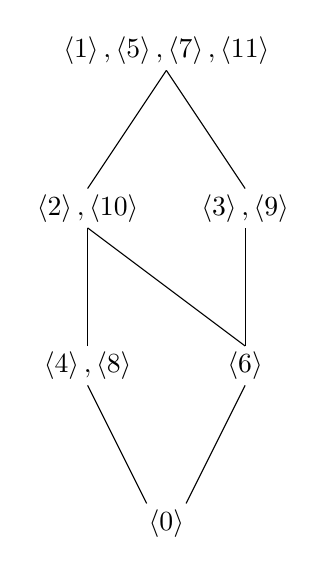
\begin{tikzpicture}
    \node at (2,6) {$\cycle{1},\cycle{5},\cycle{7},\cycle{11}$};
    \node at (1,4) {$\cycle{2},\cycle{10}$};
    \node at (3,4) {$\cycle{3},\cycle{9}$};
    \node at (1,2) {$\cycle{4},\cycle{8}$};
    \node at (3,2) {$\cycle{6}$};
    \node at (2,0) {$\cycle{0}$};
    \draw (1.75,0.25) -- (1,1.75);
    \draw (2.25,0.25) -- (3,1.75);
    \draw (1,2.25) -- (1,3.75);
    \draw (3,2.25) -- (3,3.75);
    \draw (3,2.25) -- (1,3.75);
    \draw (1,4.25) -- (2,5.75);
    \draw (3,4.25) -- (2,5.75);
  \end{tikzpicture}
\end{example}

\begin{corollary}
  Let $G=\cycle{a}$ and $\abs{G}=n$:
  \[\forall\,a^m\in G,\cycle{a^m}=\cycle{a^d},d=(m,n)\]
\end{corollary}

\begin{corollary}
  Let $G=\cycle{a}$ and $\abs{G}=n$:
  \[\forall\,a^m\in G,\abs{\cycle{a^m}}=\frac{n}{d},d=(m,n)\]
\end{corollary}

\begin{corollary}
  Let $G=\cycle{a}$ and $\abs{G}=n$:
  \[\forall\,a^m\in G,\cycle{a^m}=G\iff(m,n)=1\]
\end{corollary}

\begin{corollary}
  Let $G=\cycle{a}$ and $\abs{G}=n$:
  \[\forall\,a^h,a^k\in G,\cycle{a^h}=\cycle{a^k}\iff(h,n)=(k,n)\]
\end{corollary}

\end{document}
